% Auto-generated by the analysis pipeline — do not edit
% y > 0: Underreacts  |  y < 0: Overreacts
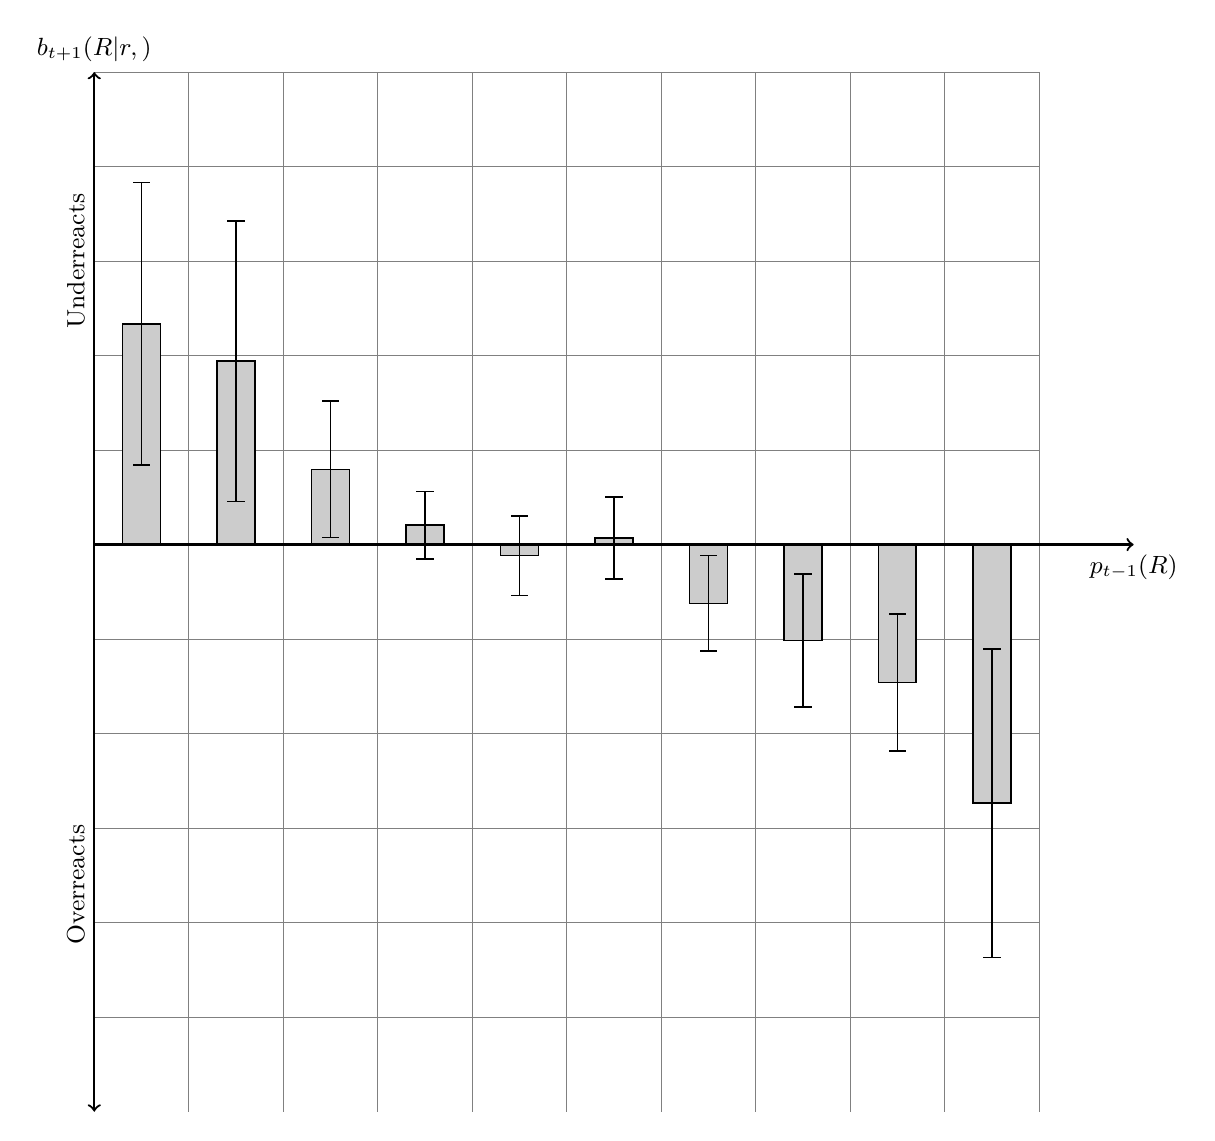
\begin{tikzpicture}[scale=12]
\draw[help lines,step=0.1] (0,-0.6) grid (1,0.5);
\filldraw[opaque,white!80!black] (0.03,0) rectangle (0.07,0.2337);
\draw[line width=0.6] (0.03,0) rectangle (0.07,0.2337);
\draw[line width=0.6,|-|] (0.05,0.0835) -- (0.05,0.3839);
\filldraw[opaque,white!80!black] (0.13,0) rectangle (0.17,0.1941);
\draw[line width=0.6] (0.13,0) rectangle (0.17,0.1941);
\draw[line width=0.6,|-|] (0.15,0.0446) -- (0.15,0.3436);
\filldraw[opaque,white!80!black] (0.23,0) rectangle (0.27,0.0796);
\draw[line width=0.6] (0.23,0) rectangle (0.27,0.0796);
\draw[line width=0.6,|-|] (0.25,0.0067) -- (0.25,0.1525);
\filldraw[opaque,white!80!black] (0.33,0) rectangle (0.37,0.0205);
\draw[line width=0.6] (0.33,0) rectangle (0.37,0.0205);
\draw[line width=0.6,|-|] (0.35,-0.0162) -- (0.35,0.0571);
\filldraw[opaque,white!80!black] (0.43,0) rectangle (0.47,-0.0117);
\draw[line width=0.6] (0.43,0) rectangle (0.47,-0.0117);
\draw[line width=0.6,|-|] (0.45,-0.0547) -- (0.45,0.0313);
\filldraw[opaque,white!80!black] (0.53,0) rectangle (0.57,0.0071);
\draw[line width=0.6] (0.53,0) rectangle (0.57,0.0071);
\draw[line width=0.6,|-|] (0.55,-0.0372) -- (0.55,0.0515);
\filldraw[opaque,white!80!black] (0.63,0) rectangle (0.67,-0.0622);
\draw[line width=0.6] (0.63,0) rectangle (0.67,-0.0622);
\draw[line width=0.6,|-|] (0.65,-0.1138) -- (0.65,-0.0106);
\filldraw[opaque,white!80!black] (0.73,0) rectangle (0.77,-0.1016);
\draw[line width=0.6] (0.73,0) rectangle (0.77,-0.1016);
\draw[line width=0.6,|-|] (0.75,-0.1728) -- (0.75,-0.0305);
\filldraw[opaque,white!80!black] (0.83,0) rectangle (0.87,-0.1458);
\draw[line width=0.6] (0.83,0) rectangle (0.87,-0.1458);
\draw[line width=0.6,|-|] (0.85,-0.2190) -- (0.85,-0.0727);
\filldraw[opaque,white!80!black] (0.93,0) rectangle (0.97,-0.2738);
\draw[line width=0.6] (0.93,0) rectangle (0.97,-0.2738);
\draw[line width=0.6,|-|] (0.95,-0.4379) -- (0.95,-0.1098);
\draw[line width=0.8,->]  (0,0) -- (1.1,0) node[below] {\small{$p_{t-1}(R)$}};
\draw[line width=0.8,<->] (0,-0.6) -- (0,0.5) node[above] {\small{$b_{t+1}(R|r,\xmark)$}};
\draw (0,0.30) node[above,rotate=90] {\small{Underreacts}};
\draw (0,-0.36) node[above,rotate=90] {\small{Overreacts}};
% ADD THEORY CURVE BELOW
\end{tikzpicture}
